\section{Environmental Impact}

\subsection{Waste prevention and minimisation}

Nitroma is conscious of the adverse effects that our activities may have on the environment. The company strives to set an industry standard for being environmentally sustainable in the chemical manufacture field. The prevention and minimisation of waste are key to achieving this goal. 

\subsubsection{Choice of reducing agent}
The selection of compounds utilised in the various plant reactions allowed waste prevention. For the hydrogenation to 4-aminobenzaldehyde and 4-aminobenzoic acid, a choice was made between two reducing agents, formic acid and ammonium formate. Whist ammonium formate is more favourable in terms of reaction time (the low residence time offering a faster pathway), the use of this reducing agent will produce ammonia as a side product. Acting as a  source of nitration pollution, gaseous ammonia emissions have harmful affects on biodiversity; forming acid deposits in soil, inflicting toxic damage on plants, and negatively altering aquatic ecosystems through a significant nutrient shift \cite{european_environment_agency_ammonia_2019}. Based on this, formic acid was chosen as the reducing agent over ammonium formate, eliminating the unnecessary formation of ammonia. 

\subsubsection{Sulphuric acid and nitrogen oxides}
The nitration reaction process presented an opportunity for waste prevention and minimisation. Traditionally, nitration reactions employ a mixture of nitric acid and sulphuric acid. However, the disposal of 'spent' sulphuric acid has been found to be both costly and environmentally unfriendly \cite{smith_superior_1996}. The replacement of sulphuric acid with the zeolite, H-Modernite, provides a more environmentally sustainable nitration pathway. H-Modernite comes with various advantages, including low catalyst loading, its ability to allow short reaction times and its reusable nature \cite{smith_superior_1996}. Another issue with the use of sulphuric acid in nitration is that it leads to decomposition of nitric acid, forming harmful nitrogen oxides (\ch{NO_x}). Upon the replacement of sulphuric acid with a zeolite catalyst, extensive research was conducted to investigate how \ch{NO_x} may be formed. Our research showed no evidence of \ch{NO_x} emissions from nitration with zeolite catalysts. Nitroma has hypothesised that there is a rapid reaction between the zeolite and the \ch{NO_x} formed from nitric acid decomposition, the resulting product being a nitrating agent which reacts in the nitration itself. Further details on can be found in the synthesis \cref{sec:NOx}. Thus, the use of H-Modernite has allowed prevention of \ch{NO_x} emissions - however if there should be \ch{NO_x} emissions, research suggests this would be less than what would be produced with sulphuric acid. If \ch{NO_x}'s are produced, it will pass through a scrubber before release (see gaseous waste treatment). Thus, through this choice, the minimisation of \ch{NO_x} production via nitration (if not its complete elimination) has been achieved. 

\subsubsection{Recycle and recovery}

Where possible, recycle streams have been integrated into the process, to recover essential reactants. Recycling is desirable as this means less pollutants within the waste streams and also less of the materials will need to be outsource, thus less spending and less indirect effect of greenhouse gas emissions via imports (see Table\ref{tab:recycle}).


\begin{table}[h]
\centering
\caption{Amount of substances recovered each year }
\label{tab:recycle}
\begin{tabular}{@{}ll@{}}
\toprule
Substance           & \begin{tabular}[c]{@{}l@{}}Amount recovered   \\      \si{tonne\per\year}\end{tabular} \\ \midrule
Formic acid         & 1158.61                                                                       \\
Hydrogen            & 63.19                                                                         \\
Methanol            & 6243.15                                                                       \\
Nitric acid         & 1439.86                                                                       \\
Toluene             & 122.26                                                                   \\
2-nitrotoluene      & 626.35                                                                        \\
4-nitrotoluene      & 615.48                                                                        \\
2-nitrobenzoic acid & 1268.07                                                              \\ \bottomrule
\end{tabular}
\end{table}


\subsection{Waste Treatment}
\label{sec:waste}


Whilst every effort has been made to prevent and minimise waste, there will inevitably be materials that must be disposed. Nitroma has considered the best techniques available to appropriately treat the various waste streams, ensuring that they comply with the imposed limits. The waste consists of mostly unreacted organic substances, along with spent nitric acid and methanol that was unable to recovered via the recycle. Nitroma will have two operations, the BA operation (in which target product is 4-aminobenzoic acid) and the BH operation (the target product being 4-aminobenzaldehyde). Each operation follows the same waste treatment, as described in this section. 


\subsubsection{Liquid waste }

Due to the continuous nature of the plant, liquid effluent streams will be continually discharged and so there must be an on-site wastewater treatment plant that is able to manage this demand sufficiently \cite{water_innovations_inc_continuous_2021}.  As seen in tables \ref{tab:wasteBA} and \ref{tab:bhwaste}, the waste streams have high organic content, which is reflected by the high chemical oxygen demand (COD) values of each substance respectively. Each of the waste streams are first collected and stored (Tables \ref{tab:wasteBA} \& \ref{tab:bhwaste}), the unit with formic acid being diluted to lower the acidic concentration. Stream 1-16, going out of the nitric acid regeneration unit, will go straight to the neutralisation unit instead of being stored, to treat the nitric acid with lime. The outlet from neutralisation will pass through a filter. Here the solid deposits will be retained and sent to landfill, whilst the filtrate will be mixed with the remaining waste streams. This stream will then be sent to the subsequent treatment units. 

Various waste treatment methods were investigated, with the performance,  safety of materials involved and economics all taken into account. Options considered included the photo-fenton-oxidation process and wet air oxidation. However these processes were deemed unsuitable due to the flammable nature of some of the components present in the waste streams, including methanol and formic acid. Ultimately, it was decided to use two methods; first adsorption using activated carbon followed by treatment in an anaerobic membrane bioreactor (AnMBR). The adsorption process is highly effective in removing organics from the waste streams, reducing the COD by over \SI{90}{\percent}. Adsorption is also capable of capturing any inorganics that may be present from the neutralisation process. The use of commercial activated carbon produced is highly favourable,  offering a high performance treatment (reducing the COD by \SI{96.4}{\percent}) \cite{aluyor_cod_2008}. Following adsorption, the organic waste stream will be sent into the AnMBR for further treatment. AnMBRs offer a low energy input treatment method for waste treatment \cite{maaz_anaerobic_2019}, allowing over \SI{98}{\percent} COD removal whilst transforming the organic matter into biogas \cite{chen_brewery_2016}. The biogas consists mainly of methane, produced via action of anaerobic microorganisms. Approximately \SI{70}{\percent} of organics are converted into methane \cite{ariunbaatar_performance_2021}, whilst the rest is broken down into \ch{CO2}. Nitroma plans to sell this biogas for energy generation, however in the future, we hope to establish a system that allows the integration of this energy for our own activities. Configurations of the AnMBR can vary, however it was decided that the membrane module will remain outside the bioreactor itself for better monitoring and maintenance \cite{maaz_anaerobic_2019}. Collaboratively, the use adsorption and AnMBR will be able to reduce the overall COD of the liquid waste effluent below the maximum limit of \SI{250}{\mg\per\litre}. 

\subsubsection{Gaseous Waste}

All the gaseous waste 
streams contain volatile organic compounds and will thus be disposed of via incineration. Whilst initially cryogenic condensation was considered as a treatment methods, it was clear that the construction and installation of this system itself would be more damaging to the environment in comparison to the amount of direct greenhouse gas emissions it would save. The complete combustion of organic compounds is assumed and thus the emission of carbon monoxide and carbon are negligible. To minimise \ch{NO_x} emissions, a low \ch{NO_x} burner will be utilised, favourable due to its \ch{NO_x} removal efficiency (\SI{74}{\percent}), along with low cost in comparison to other \ch{NO_x} removal methods such as fuel staging and gas recirculation \cite{world_bank_group_pollution_1999}. In addition to this, the flue gas will go through a wet scrubber, with a \SI{99}{\percent} efficiency for \ch{NO_x} removal \cite{ceco_environmental_nox_nodate}. Through the employment of these methods, the \ch{NO_x} emissions have been limited to 2.78kg/hr during both the BA and BH scenario, with a total of \SI{18.37}{\tonne\per\year} (for 275 days of operation a year). The total \ch{CO2} emissions have been approximated to 1082.50 t/y released, with 174.61kg/hr released during the BH scenario and 91.35kg/hr released during the BA scenario. 

To investigate the atmospheric dispersion of \ch{CO2} and \ch{NO2}, the point source Gaussian Plume model was utilised, with the following assumptions made:

\begin{itemize}
\item Constant emission rate of \ch{CO2} and \ch{NO_x} from source
\item Constant wind speed of \SI{3.8}{\m\per\s} \cite{weather_spark_average_nodate}
\item Effective stack height of \SI{25}{\m} 
\end{itemize}

\begin{equation}
C(x,0,0)= \frac{Q}{\pi u_{H} \sigma_{y} \sigma_{z}} \exp\left( \frac{H^2}{2\sigma_{z}^2}\right)
\end{equation}


The \ch{CO2} and \ch{NO2} emissions (in both the BA and the BH scenario), fall below their respective long-term workplace exposure limits (\SI{9150}{\mg\per\cubic\m} and \SI{0.96}{\mg\per\cubic\m}) at the closest proximity to the plant that are imposed under the COSHH law \cite{great_britain_health_and_safety_executive_workplace_2020}. The highest concentration of \ch{CO2} occurs during the BH operation, with a peak of \SI{1.64}{\mg\per\cubic\m}  (under the unstable condition), whilst the highest \ch{NO2} concentration is \SI{0.026}{\mg\per\cubic\m} under neutral conditions for both the BA and the BH operation (falling below the imposed maximum limit of \SI{0.04}{\mg\per\cubic\m} \cite{european_commission_standards_nodate}). 
The BH operation plume models can be seen in \ref{fig:CO2plumeBH} and \ref{fig:NO2plumeBH}. The plume models for the BA scenario are available in the appendix. When taking the $\pm \SI{50}{\percent}$ accuracy limit of the plume model into account, Nitroma is still able to guarantee compliance to all the relevant regulations.  

\begin{figure*}[t!]
    \centering
    \begin{minipage}[t]{0.5\textwidth}
        \centering
        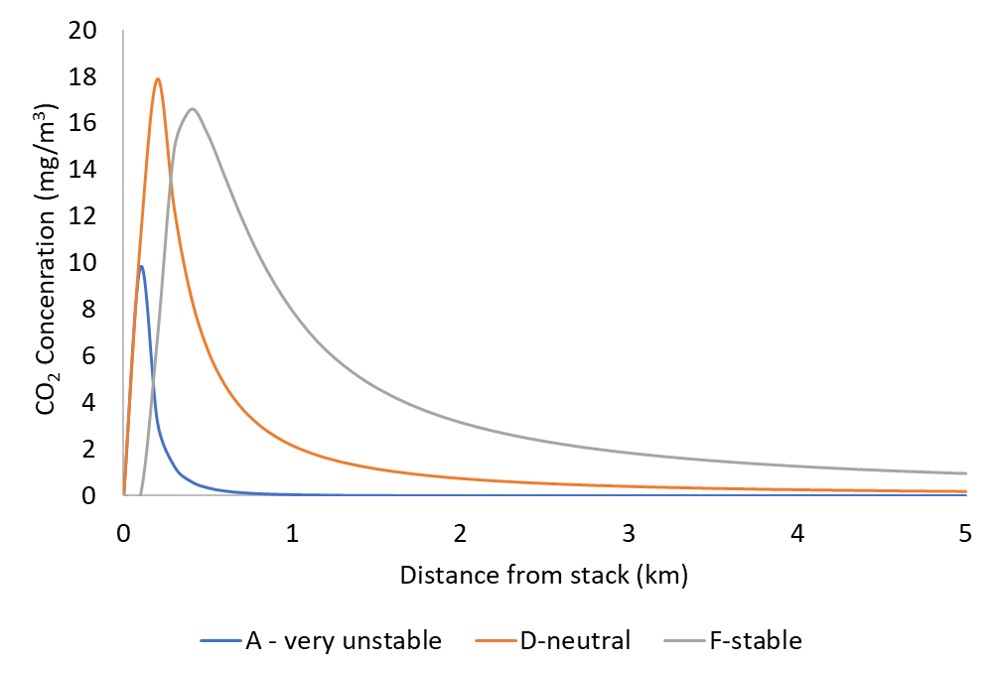
\includegraphics[width=\linewidth]{chapters/5-safety-layout-environment/figures/CO2plumeBH.jpg}
        \caption{\ch{CO2} plume model from BH scenario}
        \label{fig:CO2plumeBH}
    \end{minipage}%
    ~ 
    \begin{minipage}[t]{0.5\textwidth}
        \centering
        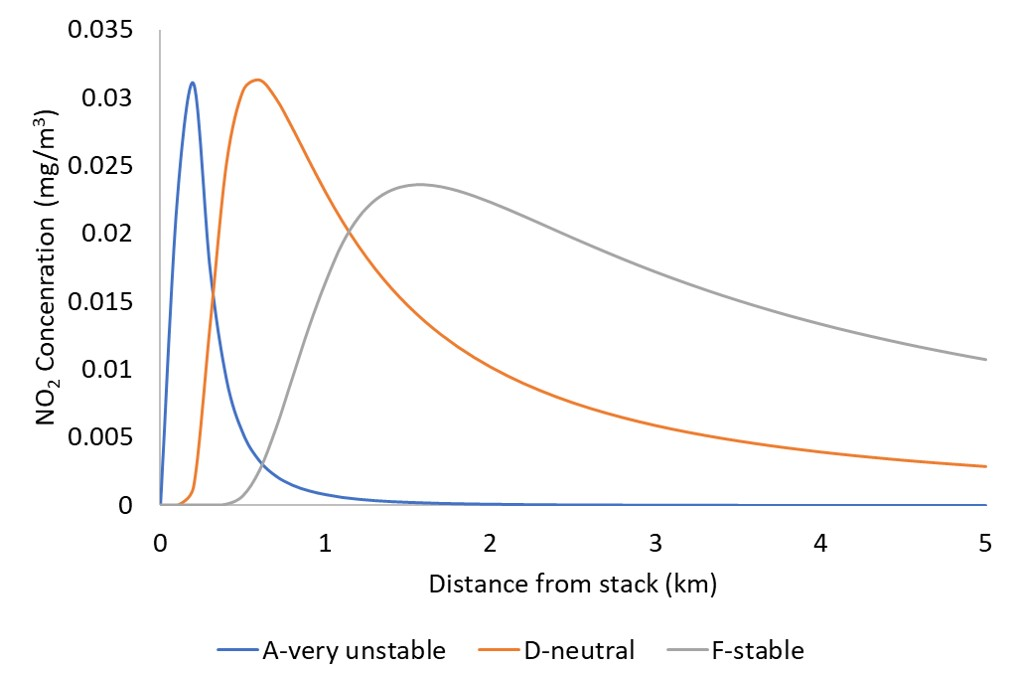
\includegraphics[width=\linewidth]{chapters/5-safety-layout-environment/figures/NO2plumeBH.jpg}
        \caption{\ch{NO2} plume model from BH scenario}
         \label{fig:NO2plumeBH}
    \end{minipage}
    
\end{figure*}


\subsection{Greenhouse Gas Emissions}

\begin{wraptable}[6]{r}{0.4\linewidth}
\vspace{-\intextsep}
\caption{Greenhouse gas emissions}
\label{tab:GHG}
\begin{tabular}{@{}lllll@{}} \toprule
Emissions (tonnes/year) & \ch{CO2}    & \ch{NO2}  \\ \midrule
Direct                  & 1082.5 & 18.4 \\
Indirect                & 8.738      &  -     \\
Total                   & 1091.2     &  18.4   \\\bottomrule
\end{tabular}
\end{wraptable}

The greenhouse gas emissions from Nitroma's plant are summarised in \cref{tab:GHG}. The direct emissions were from the incineration of waste streams in the waste treatment area and the indirect emission were from the electricity consumption in the plant for manufacturing the products. The electricity to consumed was \SI{8734.8}{\kWh\per\year}. This was converted to carbon dioxide emission using estimated average carbon intensity in Jiangsu, 2020 of \SI{0.001}{\tonne\per\kWh} \cite{li_chinas_2017}. Nitroma is also striving to become as green as possible and part of this is goal is reducing greenhouse gas emissions. The design team is constantly exploring options for greater recovery of unreacted organics, especially those within the gaseous waste streams to reduce the level of incineration that occurs. In the future Nitroma hopes to safely implement more efficient recycle system that allow this to be achieved.

\subsection{Embodied Energy}

\begin{wraptable}{r}{0.4\linewidth}
\vspace{-\intextsep}
\centering
    \caption{Embodied Energy}
    \label{tab:embodied}
\begin{tabular}{@{}lllll@{}}
\toprule
 & Embodied energy (MJ/kg)  \\ \midrule
Raw materials    & 152.76   \\
Transportation     &  0.012  \\
Production           & 0.024   \\
Total                  & 152.796   \\\bottomrule
\end{tabular}
\end{wraptable} 

Embodied energy in Nitroma's plant was estimated per kilogram of product manufactured. The energy involved in the extraction of raw material, transportation of the raw material to Nitroma's plant and finally manufacturing the final products are summarised in \cref{tab:embodied}. The embodied energy in the raw materials were approximated from OpenLCA, using Cumulative Energy Demand (CED) metric. The embodied energy in transportation was determined based on the distance travelled by heavy duty vehicles from the supplier to the plant. The embodied energy from production is the electricity consumed throughout the plant to process the final products. 



